\documentclass{beamer}
%\usetheme[style=simple,sidebar=.125\paperwidth]{Frederiksberg}
%\usetheme{Madrid} % My favorite!
%\usetheme{Boadilla} % Pretty neat, soft color.
%\usetheme{PaloAlto}  %****
%\usetheme{Hannover}  %****
%\usetheme{Montpellier}
%\usetheme{default}
\usetheme{Frankfurt}
%\usetheme{Warsaw}
%\usetheme{Bergen} % This template has nagivation on the left
%\usetheme{Frankfurt} % Similar to the default 
%with an extra region at the top.
%\usecolortheme{seahorse} % Simple and clean template
\usecolortheme{beaver}
%\usecolortheme{beetle}
%\usecolortheme{dolphin}
%\usetheme{Darmstadt} % not so good
% Uncomment the following line if you want %
% page numbers and using Warsaw theme%
% \setbeamertemplate{footline}[page number]
\setbeamercovered{transparent}
%\setbeamercovered{invisible}
% To remove the navigation symbols from 
% the bottom of slides%
\setbeamertemplate{navigation symbols}{} 
%
\mode<presentation>

%Add table of content at the beginning of each new section
\AtBeginSection[]
{
  \begin{frame}[shrink]
    \frametitle{Contents}
	\begin{scriptsize}
    \tableofcontents[currentsection]
	\end{scriptsize}
  \end{frame}
}




%iscam logo
\newcommand{\iscam}{
{$^i$}\textcolor{red}{S}\textcolor{green}{\small{}C}{\textcolor{blue}{\footnotesize{}A}}\textcolor{black}{$_\textnormal{M}$}}%{\raisebox{-0.7ex}{M}}%




\usepackage{graphicx}
\usepackage[round]{natbib}
\usepackage{array}
%\usepackage{bm}         % For typesetting bold math (not \mathbold)
\logo{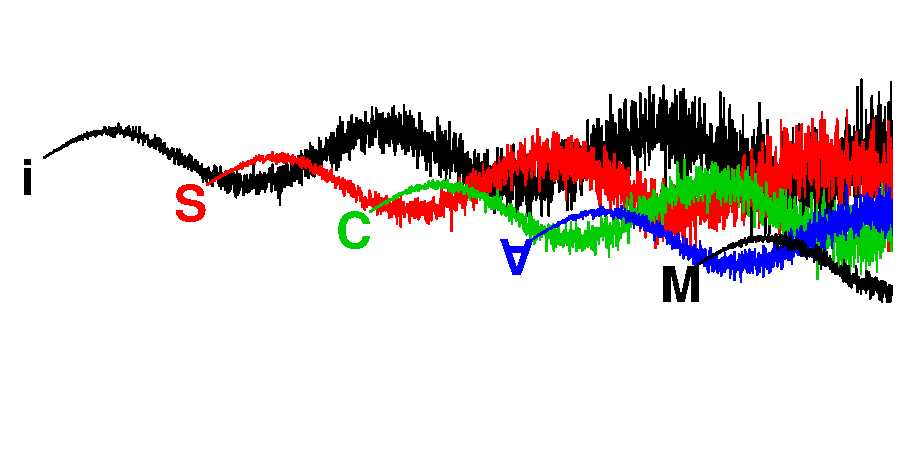
\includegraphics[height=0.6cm]{iScamLogo.pdf}}
%
\title[2011 BC Herring Assessment]{Part I: Moving towards a sustainable fisheries framework for BC herring: data, models \& alternative assumptions.\\
\vfill
Part II: Stock assessment and management advice for BC Herring stocks (2011/2012)\\}
\author{Steven Martell, Jake Schweigert, Jaclyn Cleary, Vivian Haist}
\institute[UBC]
{
University of British Columbia \\
\medskip
{\emph{martell.steve@gmail.com}}
}
\date{\today}
% \today will show current date. 
% Alternatively, you can specify a date.
%
\begin{document}
	\def\newblock{\hskip .11em plus .33em minus .07em}
%
\begin{frame}
\titlepage
\end{frame}
%



%!TEX root = /Users/stevenmartell/Documents/CURRENT PROJECTS/iSCAM-trunk/fba/BC-herring-2011/PRESENTATION/BC-Herring-2011.tex
%%%   %%%   %%%   %%%   %%%   %%%   %%%   %%%   %%%   %%%   %%%   %%%   %%%   %%%   
%% Outline for Part I
%% Sustainable Fisheries Framework.
%% 		-HCAM Review
%% 
%%%   %%%   %%%   %%%   %%%   %%%   %%%   %%%   %%%   %%%   %%%   %%%   %%%   %%%   
%%%%%%%%%%%%%%%%%%%%%%%%%%%%%%%%%%%%%%%%%%%%%%%%%%%%%
%%%%%%%%%%%%%%%%%%%%%%%%%%%%%%%%%%%%%%%%%%%%%%%%%%%%%

%%%%%%%%%%%%%%%%%%%%%%%%%%%%%%%%%%%%%%%%%%%%%%%%%%%%%
%%%%%%%%%%%%%%%%%%%%%%%%%%%%%%%%%%%%%%%%%%%%%%%%%%%%%
\section{Sustainable Fisheries Framework} % (fold)
\label{sec:sustainable_fisheries_framework}


\subsection{HCAM Review} % (fold)
\label{sub:hcam_review}

\begin{frame}[t]\frametitle{June 2010: HCAM Review Workshop}
	\begin{block}	{Terms of Reference (paraphrased)}
		\begin{itemize}
			\item<1-> Herring spawn index, is $q=1$ assumption appropriate?
			\item<1-> HCR, should CUTOFF change in concert with $B_0$ updates?
			\item<1-> What is the best way to parameterize natural mortality?
			\item<1-> Are the priors appropriate and is uncertainty appropriately reflected in assessments?
			\item<1-> Preference for selectivity/availability parameterization.
			\item<1-> Should stock assessments be conducted on a risk-neutral or risk-averse basis?
			\item<2-> Appropriate assumptions for an operating model (MSE).
		\end{itemize}
	\end{block}
\end{frame}

%
\begin{frame}[t]\frametitle{Summary of Panel Recommendations}
	\begin{enumerate}
		\item<+> Assumption that $q=1$ was inappropriate.
		\item<+> CUTOFFS can be fixed or updated annually.
		\item<+> A model based approach to estimating $B_0$ and $B_{MSY}$ is appropriate.
		\item<+> Recruitment variation $\sigma_R$ should be estimated within the model.
		\item<+> Issues regarding estimation of selectivity, natural mortality and $q$ should be explored.
		\item<+> Science advice should be risk neutral.
	\end{enumerate}
	
	\only<1>{The model parameterization of $q$ could potentially have the single greatest effect on estimation of management parameters, and as such further investigation is recommended. }
	
	\only<2>{If the intention is that the CUTOFF represents 25\% $B_0$ then it should be updated in conjunction with stock assessment updates.  }
	
	\only<3>{Estimates of MSY based reference points are sensitive to the assumed form of the recruitment model and allocation to gears with different selectivities.}
	
	\only<4>{Note that MLE estimates of $\sigma_R$ are biased; values from the joint posterior distribution are unbiased. }
\end{frame}

% subsection hcam_review (end)

\subsection{Harvest Control Rule} % (fold)
\label{sub:harvest_control_rule}
\begin{frame}[t]\frametitle{Current Harvest Control Rule}
	\begin{columns}
		\begin{column}[c]{0.5\textwidth}
			\begin{itemize}
				\item  CUTOFF set at 0.25 $B_0$ (last updated in 1996).
				\item 20\% exploitation rate.
				\item Forecast based on poor, average, good recruitment.
			\end{itemize}
	\end{column}
	\begin{column}[c]{0.5\textwidth}
		\begin{figure}[htbp]
			\centering
				\includegraphics[scale=.35]{../FIGS/Herring_HCR}
			\caption{HCR for herring stocks.}
			\label{fig:Herring_HCR}
		\end{figure}
	\end{column}
	\end{columns}
\end{frame}
% subsection harvest_control_rule (end)

\subsection{Precautionary Approach} % (fold)
\label{sub:precautionary_approach}
\begin{frame}
	\frametitle{Harvest Strategy Compliant with Precautionary Approach} 
	\begin{figure}
		[htbp] \centering 
		\includegraphics[width=0.7
		\textwidth]{SSF} \caption{Fisheries management framework consistent with a precautionary approach.} \label{fig:SSF} 
	\end{figure}
\end{frame}

%
\begin{frame}
	\frametitle{Key elements for the new framework} 
	\begin{block}
		{Reference points} 
		\begin{itemize}
			\item Limit Reference Point (LRP) \& Upper Stock Reference (USR) requires knowledge of stock productivity and population scale. 
			\item Removal Rate requires knowledge of stock productivity. 
			\item MSY-based reference points require \textit{a priori} allocation to different gears. 
		\end{itemize}
	\end{block}
	\begin{block}
		{Risk \& Decision making} 
		\begin{itemize}
			\item Onus on being able to reliably determine stock status (informative data). 
		\end{itemize}
	\end{block}
\end{frame}
% subsection precautionary_approach (end)



% section sustainable_fisheries_framework (end)
%%_________________________________________________%%

%%%%%%%%%%%%%%%%%%%%%%%%%%%%%%%%%%%%%%%%%%%%%%%%%%%%%
%%%%%%%%%%%%%%%%%%%%%%%%%%%%%%%%%%%%%%%%%%%%%%%%%%%%%
\section{Part I} % (fold)
\label{sec:part_i}
%
\subsection{Analytical Methods} % (fold)
\label{sub:analytical_methods}
%
\subsubsection{Input Data} % (fold)
\label{ssec:inputdata}
%
\begin{frame}
	{Input data} The input data for \iscam\ is the same as HCAM: 
	\begin{itemize}
		\item Catch by gear, 
		\item Spawn survey index, 
		\item Age-composition data for all gears, 
		\item Empirical weight-at-age data. 
	\end{itemize}
\end{frame}
%%% subsubsection inputdata (end)

\subsubsection{Model description} % (fold)
\label{ssub:model_description}
%
\begin{frame} {Integrated Statistical Catch Age Model (\iscam)} 
	
		\begin{itemize}
			\item The model is based on a statistical catch-age framework first developed by \cite{fournier1982general}.
			
			\item Flexible options for modelling selectivity, natural mortality, \& survey catchability.
			
			\item Integrated framework: joint estimation of policy parameters (e.g., reference pionts).
			\item Model is implemented in AD Model Builder \cite{ADMB2009}, and the source code is maintained at:  \url{http://code.google.com/p/iscam-project/}
		\end{itemize}

\end{frame}
%
\begin{frame}[t,allowframebreaks]\frametitle{Assumptions}
	\begin{block}
		{Error distributions}
		\begin{itemize}
			\item Observation errors in catch are lognormal \& $\sigma$ is known.
			\item Errors in spawn survey are lognormal \& $\sigma$ is unknown.
			\item Recruitment deviations are lognormal \& $\sigma$ is unknown.
			\item Age-composition residuals follow a multivariate-logistic distribution.
		\end{itemize}
	\end{block}
	
	\begin{block}
		{Selectivity}
		\begin{itemize}
			\item Seine gears: asymptotic and time invariant.
			\item Gillnet gear: parametric logistic function with weight anomalies as a covariate. 
		\end{itemize}
	\end{block}
	
	\framebreak
	\begin{block}
		{Structural assumptions}
		\begin{itemize}
			\item Age-2 recruitment with a Beverton-Holt model.
			\item Fishing \& natural mortality occur simultaneously (Baranov catch equation).
			\item Natural mortality is age-independent.
			\item Natural mortality can vary over time (random walk, $\sigma=0.1$).
			\item 100\% of the total mortality occurs before spawning.
			\item Fecundity is proportional to mature biomass.
		\end{itemize}
	\end{block}
	
	\begin{block}
		{Equilibrium \& MSY-based reference points}
		\begin{itemize}
			\item $B_o$ is based on average $M$ and average fecundity-at-age.
			\item $B_{MSY}$ is based on average ($M$) and \underline{fecundity in terminal year}.
		\end{itemize}
	\end{block}
	
\end{frame}

\begin{frame}[c]\frametitle{Objective function}
	
		Major components of the objective function
		\begin{enumerate}
			\item Likelihoods for data.
			\item Likelihoods for structural assumptions.
			\item Phased penalties to ensure regular solution.
			\item Prior densities for model parameters.
		\end{enumerate}
\end{frame}
%
\begin{frame}[c]\frametitle{Likelihoods for data}

		\begin{itemize}
			\item<+-> Normal density functions for:
			\begin{itemize}
				\item catch residuals (log-scale) with fixed $\sigma^2$,
				\item spawn survey residuals (log-scale) with estimated $\sigma^2$. 
			\end{itemize}
			\vfill
			\item<+-> Multivariate logistic function for age-composition evaluated at the conditional MLE of $\sigma^2$.
			\begin{itemize}
				\item age-proportions $<$ 2\% are pooled into adjacent age class. 
			\end{itemize}
		\end{itemize}
\end{frame}
%
\begin{frame}[c]\frametitle{Structural Assumptions}
		\begin{itemize}
			\item<+-> Stock-recruitment \\ 
			\begin{align}
				\ln\ell &= n\ln(\tau) + \frac{\sum_t \delta_t^2}{2\tau^2},\nonumber\\
				\delta_t &= \ln(N_{2,t}) - \ln(f(SB_t))\nonumber
			\end{align}
			\item<+-> Natural mortality (random walk)\\
			\begin{align}
				M_{t+1} &= M_t \exp(\varphi_t) \nonumber \\
				\ln\ell &= n\ln(\sigma) + \frac{\sum_{t=2}^T (\varphi_t-\varphi_{t-1})^2}{2\sigma^2}\nonumber
			\end{align}
		\end{itemize}
\end{frame}
%
\begin{frame}[c]\frametitle{Phased Penalties}
		\begin{itemize}
			\item<+->  Mean fishing mortality rate:
			\[  \ln(\sigma_{\bar{F}}) + \frac{(\ln(\bar{F})-\ln(0.2))^2}{2\sigma_{\bar{F}}^2},
			\quad \sigma_{\bar{F}}^{(1-3)}=0.05, \quad \sigma_{\bar{F}}^{(4)}=2.0  \]
			
			\item<+-> Deviations in average recruitment:
			\begin{align}
				\ln(\sigma_{\omega}) + \frac{\sum_t\omega_t^2}{2\sigma_{\omega}^2},
				\quad \sigma_{\omega}^{(1-3)}=0.0707, \quad \sigma_{\omega}^{(4)}=2.0 \nonumber\\
				%
				\ln(\sigma_{\ddot{\omega}}) + \frac{\sum_t\ddot{\omega}_t^2}{2\sigma_{\ddot{\omega}}^2},
				\quad \sigma_{\ddot{\omega}}^{(1-3)}=0.0707, \quad \sigma_{\ddot{\omega}}^{(4)}=2.0\nonumber
			\end{align}
		\end{itemize}
\end{frame}
%
\begin{frame}[c,allowframebreaks]\frametitle{Priors}
	
	\begin{table}
	\caption{Prior distributions for key model parameters.}
	\begin{tabular}{cccc}
		\hline
		Parameter & Distribution  & P1 & P2 \\
		\hline
		$\ln(R_0)$ & Uniform &  -5.0 & 15 \\
		Steepness & Beta &  10.0 & 4.925373\\
		Natural mortality ($\ln(M)$) &  Normal &   -0.7985077 & 0.2\\
		Rbar & Uniform &  -5.0 & 15 \\
		Rinit & Uniform &   -5.0 & 15 \\
		Variance ratio ($\rho$) & Beta & 17.08696 & 39.0559 \\
		Precision & Gamma &  25.0 & 28.75\\
		Survey $\ln(q)$ &Normal &  -0.569 & 0.274\\
		\hline
	\end{tabular}	
	\end{table}
	
	\begin{figure}[htbp]
		\centering
		\includegraphics[width=0.7\textwidth]{../FIGS/qPriorFigs/iscam_fig_theta_prior_density.pdf}
		\caption{Prior densities for leading model parameters.}
		\label{fig:priors}
	\end{figure}
\end{frame}

%%% subsubsection model_description (end)

%% subsection analytical_methods (end)

%
\subsection{Simulation testing} % (fold)
\label{sub:simulation_testing}
\begin{frame}[t]\frametitle{Simulation testing}
	Estimation performance with perfect information.\\
	\begin{center}
		\only<1>{
		\includegraphics[clip,trim=0 225 260 0,height=0.8\textheight]{../FIGS/simplot}
		}
		\only<2>{
		\includegraphics[clip,trim=0 0 260 225,height=0.8\textheight]{../FIGS/simplot}
		}
		\only<3>{
		\includegraphics[clip,trim=275 225 0 0,height=0.8\textheight]{../FIGS/simplot}
		}
	\end{center}
	

\end{frame}
%
\begin{frame}[t]\frametitle{Precision \& Bias}
	Bias ratios for key model parameters based on 50 simulated data sets.
	\begin{center}
		\only<1>{
		\includegraphics[clip,trim= 0 250 0 0, width=\textwidth]{../FIGS/SOGparameterBias}
		}
		\only<2>{
		\includegraphics[clip,trim= 0 0 0 220, width=\textwidth]{../FIGS/SOGparameterBias}
		}
	\end{center}
 
\end{frame}
%% subsection simulation_testing (end)

\subsection{SOG Comparison} % (fold)
\label{sub:sog_comparison}
\begin{frame}[t]\frametitle{Strait of Georgia}
	Objective: set up \iscam\ $\sim$ HCAM \& compare.
	\begin{alertblock}
		{Significant differences between \iscam\ \& HCAM}
		\begin{itemize}
			\item<+-> Likelihood for age-comps.
			\item<1-> Pooling of age-proportions less than 2\% into adjacent cohort.
			\item<+-> Conditional MLE for survey $q$.
			\item<+-> Estimation of total variance and variance partitioning parameter ($\vartheta, \rho$).
			\item<+-> Prior for steepness ($h \sim$ Beta in \iscam)
		\end{itemize}
	\end{alertblock}
\end{frame}
%
\begin{frame}[c]\frametitle{SOG Spawning biomass}
	\only<1>{
	\begin{figure}[htbp]
		\centering
			\includegraphics[clip,trim=25 315 270 18,width=\textwidth]
			{../FIGS/iscam_fig_HCAM_SOG_MLE}
		\caption{Total biomass at the start of the year, spawning biomass after fishing. HCAM (2010) spawning biomass shown in red.}
	\end{figure}
	}
	
	\only<2>{
	\begin{figure}[htbp]
		\centering
			\includegraphics[clip,trim=290 30 0 305,width=\textwidth]
			{../FIGS/iscam_fig_HCAM_SOG_MLE}
		\caption{Observed and predicted spawn survey data for surface (black) and dive (red) surveys.}
	\end{figure}
	}
	
\end{frame}
%% subsection sog_comparison (end)

\subsection{Spawning biomass in major areas} % (fold)
\label{sub:spawning_biomass_in_major_areas}
\begin{frame}[c]
	\only<1>{
	\frametitle{Spawning biomass in HG}
	\includegraphics[clip,trim=0cm 10.773cm 9.775cm 0cm]
	{../FIGS/iscam_fig_SBt_iSCAMvsHCAM}
	}
	%
	\only<2>{
	\frametitle{Spawning biomass in PRD}
	\includegraphics[clip,trim=0cm 5.7cm 9.775cm 5.1cm]
	{../FIGS/iscam_fig_SBt_iSCAMvsHCAM}
	}
	%
	\only<3>{
	\frametitle{Spawning biomass in CC}
	\includegraphics[clip,trim=0cm 0cm 9.775cm 10.4cm]
	{../FIGS/iscam_fig_SBt_iSCAMvsHCAM}
	}
	%
	\only<4>{
	\frametitle{Spawning biomass in SOG}
	\includegraphics[clip,trim=9.775cm 10.773cm 0cm 0cm]
	{../FIGS/iscam_fig_SBt_iSCAMvsHCAM}
	}
	%
	\only<5>{
	\frametitle{Spawning biomass in WCVI}
	\includegraphics[clip,trim=9.775cm 5.7cm 0cm 5.1cm]
	{../FIGS/iscam_fig_SBt_iSCAMvsHCAM}
	}
\end{frame}
% subsection spawning_biomass_in_major_areas (end)

\subsection{Discussion} % (fold)
\label{sub:discussion}
\begin{frame}[t]\frametitle{Discussion}
	\begin{itemize}
		\item<+-> Slight bias in MSY reference points and steepness; likely due to lack of contrast in simulated data.
		\item<+-> Despite differences between assessment platforms there is a remarkable correspondence in spawning biomass estimates.
		
		\item<+-> Significant differences in:
		\begin{itemize}
			\item weighting of age-composition data,
			\item pooling of age-composition samples ($<$2\%),
			\item conditional MLE for dive survey $q$ with a very informative prior,
			\item prior for steepness.
		\end{itemize}
		\item<+-> MSY based reference points require unbiased estimates of selectivity parameters, and allocation of catch to each gear must be established \textit{a priori}.
	\end{itemize}
\end{frame}
%% subsection discussion (end)
% section part_i (end)
%%_________________________________________________%%
























%!TEX root = /Users/stevenmartell/Documents/CURRENT PROJECTS/iSCAM-trunk/fba/BC-herring-2011/PRESENTATION/BC-Herring-2011.tex

\section{Part II} % (fold)
\label{sec:part_ii}

\subsection{Introduction} % (fold)
\label{sub:introduction}
%
\begin{frame}[t]\frametitle{Introduction}
	Objectives:
	\begin{enumerate}
		\item Data used in the 2011 assessment.
		\item Overview of the analytical methods.
		\item Present the 2011 stock assessment.
		\item Describe \& present the catch forecasts for 2012.
	\end{enumerate}
\end{frame}

%% subsection introduction (end)

\subsection{2011 Data} % (fold)
\label{sub:2011_data}
%
\begin{frame}[c]\frametitle{Data used in the 2011 stock assessment}
	\begin{itemize}
		\item Catch by gear type.
		\item Spawn survey data.
		\item Age-composition data.
		\item Empirical weight-at-age data. 
	\end{itemize}
\end{frame}
%
\begin{frame}[t]\frametitle{Catch by gear (1950:2011)}
	\only<1>{
	\begin{figure}[htbp]
		\centering
		\includegraphics[clip,trim=0 304 300 0 ]
		{../FIGS/iscam_fig_CatchMajorAreas}
		\caption{Catch by gear for Haida Gwaii.}
	\end{figure}
	}
	\only<2>{
	\begin{figure}[htbp]
		\centering
		\includegraphics[clip,trim=0 156 300 155 ]
		{../FIGS/iscam_fig_CatchMajorAreas}
		\caption{Catch by gear for Prince Rupert District.}
	\end{figure}
	}
	\only<3>{
	\begin{figure}[htbp]
		\centering
		\includegraphics[clip,trim=0 0 300 301 ]
		{../FIGS/iscam_fig_CatchMajorAreas}
		\caption{Catch by gear for Central Coast.}
	\end{figure}
	}
	\only<4>{
	\begin{figure}[htbp]
		\centering
		\includegraphics[clip,trim=300 304 0 0 ]
		{../FIGS/iscam_fig_CatchMajorAreas}
		\caption{Catch by gear for Strait of Georgia.}
	\end{figure}
	}
	\only<5>{
	\begin{figure}[htbp]
		\centering
		\includegraphics[clip,trim=300 156 0 155 ]
		{../FIGS/iscam_fig_CatchMajorAreas}
		\caption{Catch by gear for West Coast of Vancouver Island.}
	\end{figure}
	}
\end{frame}
%
\begin{frame}[t]\frametitle{Spawning activity in 2010}
	\only<1>{
	\begin{figure}[htbp]
		\centering
		\includegraphics[scale=0.23]
		{../FIGS/PBSfigs/2011_spawn_HG_2E_July13}
		\includegraphics[scale=0.23]
		{../FIGS/PBSfigs/2011_spawn_HG_2W_July13}
		%{../FIGS/PBSfigs/2011-HG-Prelim-WG}
		\caption{2010 Spawning activity in Haida Gwaii.}
	\end{figure}
	}
	\only<2>{
	\begin{figure}[htbp]
		\centering
		\includegraphics[scale=0.23]
		{../FIGS/PBSfigs/2011_spawn_PRD_July13}
		\caption{2010 Spawning activity in Prince Rupert District.}
	\end{figure}
	}
	\only<3>{
	\begin{figure}[htbp]
		\centering
		\includegraphics[scale=0.23]
		{../FIGS/PBSfigs/2011_spawn_CCJuly13}
		\caption{2010 Spawning activity in Central Coast.}
	\end{figure}
	}
	\only<4>{
	\begin{figure}[htbp]
		\centering
		\includegraphics[scale=0.23]
		{../FIGS/PBSfigs/2011_spawn_SOG_July13}
		\caption{2010 Spawning activity in Strait of Georgia.}
	\end{figure}
	}
	\only<5>{
	\begin{figure}[htbp]
		\centering
		\includegraphics[scale=0.23]
		{../FIGS/PBSfigs/2011_spawn_WCVI_August16}
		\caption{2010 Spawning activity in West Coast Vancouver Island.}
	\end{figure}
	}
\end{frame}
%
\begin{frame}[t]\frametitle{Spawn survey time series}
	\only<1>{
	\begin{figure}[htbp]
		\centering
		\includegraphics[clip,trim=0 304 275 0]
		{../FIGS/iscam_fig_SurveyMajorAreas}
		\caption{Spawn survey series in Haida Gwaii.}
	\end{figure}
	}
	%
	\only<2>{
	\begin{figure}[htbp]
		\centering
		\includegraphics[clip,trim=0 156 275 155]
		{../FIGS/iscam_fig_SurveyMajorAreas}
		\caption{Spawn survey series in Prince Rupert District.}
	\end{figure}
	}
	%
	\only<3>{
	\begin{figure}[htbp]
		\centering
		\includegraphics[clip,trim=0 0 275 301]
		{../FIGS/iscam_fig_SurveyMajorAreas}
		\caption{Spawn survey series in Central Coast.}
	\end{figure}
	}
	%
	\only<4>{
	\begin{figure}[htbp]
		\centering
		\includegraphics[clip,trim=275 304 0 0]
		{../FIGS/iscam_fig_SurveyMajorAreas}
		\caption{Spawn survey series in Strait of Georgia.}
	\end{figure}
	}
	%
	\only<5>{
	\begin{figure}[htbp]
		\centering
		\includegraphics[clip,trim=275 156 0 155]
		{../FIGS/iscam_fig_SurveyMajorAreas}
		\caption{Spawn survey series in West Coast of Vancouver Island.}
	\end{figure}
	}
\end{frame}
%
\begin{frame}[t]\frametitle{Age-composition data}
	\only<1>{
	\begin{figure}[htbp]
		\centering
		\vspace{-0.5cm}	\includegraphics
		[height=0.85\textheight,width=\textwidth]
		{../FIGS/iscam_fig_AgeCompsHG}
		\vspace{-1cm}
		\caption{Haida Gwaii: winter seine, seine-roe, gillnet.}
	\end{figure}
	}
	%
	\only<2>{
	\begin{figure}[htbp]
		\centering
		\vspace{-0.5cm}	\includegraphics
		[height=0.85\textheight,width=\textwidth]
		{../FIGS/iscam_fig_AgeCompsPRD}
		\vspace{-1cm}
		\caption{Prince Rupert District: winter seine, seine-roe, gillnet.}
	\end{figure}
	}
	%
	\only<3>{
	\begin{figure}[htbp]
		\centering
		\vspace{-0.5cm}	\includegraphics
		[height=0.85\textheight,width=\textwidth]
		{../FIGS/iscam_fig_AgeCompsCC}
		\vspace{-1cm}
		\caption{Central Coast: winter seine, seine-roe, gillnet.}
	\end{figure}
	}
	%
	\only<4>{
	\begin{figure}[htbp]
		\centering
		\vspace{-0.5cm}	\includegraphics
		[height=0.85\textheight,width=\textwidth]
		{../FIGS/iscam_fig_AgeCompsSOG}
		\vspace{-1cm}
		\caption{Strait of Georgia: winter seine, seine-roe, gillnet.}
	\end{figure}
	}
	%
	\only<5>{
	\begin{figure}[htbp]
		\centering
		\vspace{-0.5cm}	\includegraphics
		[height=0.85\textheight,width=\textwidth]
		{../FIGS/iscam_fig_AgeCompsWCVI}
		\vspace{-1cm}
		\caption{West Coast Vancouver Island: winter seine, seine-roe, gillnet.}
	\end{figure}
	}
	
\end{frame}
%
\begin{frame}[t]\frametitle{Weight-at-age}
	\only<1>{
	\begin{figure}[htbp]
		\centering
		\includegraphics[scale=0.4]
		{../FIGS/iscam_fig_weight-at-age_HG}
		\caption{Haida Gwaii: empirical weight-at-age (kg).}
	\end{figure}
	}
	%
	\only<2>{
	\begin{figure}[htbp]
		\centering
		\includegraphics[scale=0.4]
		{../FIGS/iscam_fig_weight-at-age_PRD}
		\caption{Prince Rupert District: empirical weight-at-age (kg).}
	\end{figure}
	}
	%
	\only<3>{
	\begin{figure}[htbp]
		\centering
		\includegraphics[scale=0.4]
		{../FIGS/iscam_fig_weight-at-age_CC}
		\caption{Central Coast: empirical weight-at-age (kg).}
	\end{figure}
	}
	%
	\only<4>{
	\begin{figure}[htbp]
		\centering
		\includegraphics[scale=0.4]
		{../FIGS/iscam_fig_weight-at-age_SOG}
		\caption{Strait of Georgia: empirical weight-at-age (kg).}
	\end{figure}
	}
	%
	\only<5>{
	\begin{figure}[htbp]
		\centering
		\includegraphics[scale=0.4]
		{../FIGS/iscam_fig_weight-at-age_WCVI}
		\caption{West Coast Vancouver Island: empirical weight-at-age (kg).}
	\end{figure}
	}
	%
\end{frame}
%
% subsection 2011_data (end)

\subsection{Analytical Methods} % (fold)
\label{sub:analytical_methods}
\begin{frame}[t]\frametitle{Analytics \& assumptions}
	\begin{itemize}
		\item<+-> All major and minor areas were assessed using  \iscam.
		\item<+-> Reported catch: CV = 0.005
		\item<+-> Spawn survey: proportional \& 100\% of $Z_t$.
		\item<+-> Dive survey more precise than surface survey.
		\item<+-> Fecundity $\propto$ mature weight-at-age.
		\item<+-> Seine gears: selectivity is asymptotic and time-invariant. 
		\item<+-|alert@+> Gillnet gear: logistic selectivity with weigth-at-age covariates.
		\item<+-|alert@+> $P(\ln(q_1),\ln(q_2)) \sim $ Normal($\mu=-0.569,\sigma=0.274$).
		\item<+-> Homogenous errors in age-composition (multivariate logistic).
		\item<+-> Age-samples $<$0.02 pooled in adjacent cohort.
	\end{itemize}
\end{frame}

\begin{frame}[c]\frametitle{Diagnostics, Forecasts \& Catch Advice}
	\begin{description}
		\item<+->[Diagnostics] Retrospective analysis (sequential removal of the last 10 years of data).
		\item<+->[Forecasts] One-year projection of 3+ biomass with poor, average, good age-3 recruitment.
		\item<+->[Catch advice] Based on HCR with 20\% harvest rate if above cutoff.
	\end{description}
\end{frame}
% subsection analytical_methods (end)

\subsection{Maximum Likelihood Estimates} % (fold)
\label{sub:maximum_likelihood_estimates}
%
\begin{frame}[t]\frametitle{MLE: Spawn survey}
	\only<1>{
	\begin{figure}[htbp]
		\centering
		\vspace{-1cm}
		\includegraphics[scale=0.4]
	{../FIGS/qPriorFigs/iscam_fig_survey_fit_HG}
		\vspace{-1cm}
		\caption{Haida Gwaii}
	\end{figure}
	}
	%
	\only<2>{
	\begin{figure}[htbp]
		\centering
		\vspace{-1cm}
		\includegraphics[scale=0.4]
	{../FIGS/qPriorFigs/iscam_fig_survey_fit_PRD}
		\vspace{-1cm}
		\caption{Prince Rupert District}
	\end{figure}
	}
	%
	\only<3>{
	\begin{figure}[htbp]
		\centering
		\vspace{-1cm}
		\includegraphics[scale=0.4]
	{../FIGS/qPriorFigs/iscam_fig_survey_fit_CC}
		\vspace{-1cm}
		\caption{Central Coast}
	\end{figure}
	}
	%
	\only<4>{
	\begin{figure}[htbp]
		\centering
		\vspace{-1cm}
		\includegraphics[scale=0.4]
	{../FIGS/qPriorFigs/iscam_fig_survey_fit_SOG}
		\vspace{-1cm}
		\caption{Strait of Georgia}
	\end{figure}
	}
	%
	\only<5>{
	\begin{figure}[htbp]
		\centering
		\vspace{-1cm}
		\includegraphics[scale=0.4]
	{../FIGS/qPriorFigs/iscam_fig_survey_fit_WCVI}
		\vspace{-1cm}
		\caption{West Coast Vancouver Island}
	\end{figure}
	}
	%
\end{frame}
%
\begin{frame}[t]\frametitle{MLE: Residuals in age composition data}
	\only<1>{
	\begin{figure}[htbp]
		\centering
		\vspace{-.75cm}
		\includegraphics[scale=0.5]
	{../FIGS/qPriorFigs/iscam_fig_agecompsresid_HG}
		\vspace{-1cm}
		\caption{Haida Gwaii}
	\end{figure}
	}
	%
	\only<2>{
	\begin{figure}[htbp]
		\centering
		\vspace{-.75cm}
		\includegraphics[scale=0.5]
	{../FIGS/qPriorFigs/iscam_fig_agecompsresid_PRD}
		\vspace{-1cm}
		\caption{Prince Rupert District}
	\end{figure}
	}
	%
	\only<3>{
	\begin{figure}[htbp]
		\centering
		\vspace{-.75cm}
		\includegraphics[scale=0.5]
	{../FIGS/qPriorFigs/iscam_fig_agecompsresid_CC}
		\vspace{-1cm}
		\caption{Central Coast}
	\end{figure}
	}
	%
	\only<4>{
	\begin{figure}[htbp]
		\centering
		\vspace{-.75cm}
		\includegraphics[scale=0.5]
	{../FIGS/qPriorFigs/iscam_fig_agecompsresid_SOG}
		\vspace{-1cm}
		\caption{Strait of Georgia}
	\end{figure}
	}
	%
	\only<5>{
	\begin{figure}[htbp]
		\centering
		\vspace{-.75cm}
		\includegraphics[scale=0.5]
	{../FIGS/qPriorFigs/iscam_fig_agecompsresid_WCVI}
		\vspace{-1cm}
		\caption{West Coast Vancouver Island}
	\end{figure}
	}
	%
\end{frame}
%
\begin{frame}[t]\frametitle{MLE: Mortality}
	\only<1>{
	\begin{figure}[htbp]
		\centering
		\vspace{-1cm}
		\includegraphics[scale=0.4]
	{../FIGS/qPriorFigs/iscam_fig_mortality_HG}
		\vspace{-1cm}
		\caption{Haida Gwaii}
	\end{figure}
	}
	%
	\only<2>{
	\begin{figure}[htbp]
		\centering
		\vspace{-1cm}
		\includegraphics[scale=0.4]
	{../FIGS/qPriorFigs/iscam_fig_mortality_PRD}
		\vspace{-1cm}
		\caption{Prince Rupert District}
	\end{figure}
	}
	%
	\only<3>{
	\begin{figure}[htbp]
		\centering
		\vspace{-1cm}
		\includegraphics[scale=0.4]
	{../FIGS/qPriorFigs/iscam_fig_mortality_CC}
		\vspace{-1cm}
		\caption{Central Coast}
	\end{figure}
	}
	%
	\only<4>{
	\begin{figure}[htbp]
		\centering
		\vspace{-1cm}
		\includegraphics[scale=0.4]
	{../FIGS/qPriorFigs/iscam_fig_mortality_SOG}
		\vspace{-1cm}
		\caption{Strait of Georgia}
	\end{figure}
	}
	%
	\only<5>{
	\begin{figure}[htbp]
		\centering
		\vspace{-1cm}
		\includegraphics[scale=0.4]
	{../FIGS/qPriorFigs/iscam_fig_mortality_WCVI}
		\vspace{-1cm}
		\caption{West Coast Vancouver Island}
	\end{figure}
	}
	%
\end{frame}
%
\begin{frame}[t]\frametitle{Age-2 recruits}
	\begin{figure}[htbp]
		\centering
		\vspace{-1cm}	\includegraphics[scale=0.5]{../FIGS/qPriorFigs/iscam_fig_recruitment}
		\vspace{-1cm}
		\caption{Age-2 recruits with 0.33 and 0.66 quantiles.}
	\end{figure}
\end{frame}
%% subsection maximum_likelihood_estimates (end)

\subsection{Diagnostics} % (fold)
\label{sub:diagnostics}
%
\begin{frame}[t]\frametitle{Diagnostics: Retrospective plots}
	\begin{figure}[htbp]
		\centering
		\vspace{-.75cm}	\includegraphics[scale=0.45]{../FIGS/qPriorFigs/iscam_fig_sbt_retrospective}	
		\vspace{-1cm}
		\caption{Retrospective estimates of spawning biomass.}
	\end{figure}
\end{frame}
%
\begin{frame}[t]\frametitle{Diagnostics: Trace plots}
	\begin{figure}[htbp]
		\centering
		\vspace{-0.75cm}	\includegraphics[scale=0.35]{../FIGS/qPriorFigs/iscam_fig_trace_SOG}
		\vspace{-0.65cm}
		\caption{Posterior samples: 1 million, thin 500, Strait of Georgia}
	\end{figure}
	
\end{frame}
%
\begin{frame}[t]\frametitle{Diagnostics: Pair plots}
	\begin{figure}[htbp]
		\centering
		\vspace{-1cm}	\includegraphics[scale=0.4]
		{../FIGS/qPriorFigs/iscam_fig_pairs_SOG}
		\vspace{-0.85cm}
		\caption{Posterior samples from leading parameters \& derived variables.}
	\end{figure}
\end{frame}
%
\begin{frame}[t]\frametitle{Diagnositcs: Marginal posteriors}
	\begin{figure}[htbp]
		\centering
			\includegraphics[scale=0.4]{../FIGS/qPriorFigs/iscam_fig_marginals_SOG}
		\caption{Strait of Georgia: Marginal \& prior distributions.}
	\end{figure}
\end{frame}
%% subsection diagnostics (end)

\subsection{Advice for management} % (fold)
\label{sub:advice_for_management}
\begin{frame}[t]\frametitle{Uncertainty in 2011 spawning biomass}
	\only<1>{
	\begin{figure}[htbp]
		\centering
			\includegraphics[scale=0.35]
			{../FIGS/qPriorFigs/iscam_fig_2011_SBt_posteriors}
		\caption{Marginal posterior distributions for 2011 spawning biomass.}
	\end{figure}
	}
	%
	\only<2>{
	\begin{figure}[htbp]
		\centering
			\includegraphics[scale=0.35]
			{../FIGS/qPriorFigs/iscam_fig_2011_depletion_posteriors}
		\caption{Marginal posterior distributions for 2011 spawning biomass depletion.}
	\end{figure}
	}
	%
	\only<3>{
	\begin{table}
		\caption{Estimates of 2011 spawning biomass, $B_0$, and depletion.}
		\begin{center}
		\begin{tiny}
		\begin{tabular}{l>{\bfseries}ccc|>{\bfseries}ccc|>{\bfseries}ccc}
		\hline 
		&\multicolumn{3}{c}{$SB_{2011}$} 
		&\multicolumn{3}{c}{$B_0$} 
		&\multicolumn{3}{c}{$SB_{2011}/B_0$}\\
		Stock 
		&Median & 2.5\% & 97.5\%
		&Median & 2.5\% & 97.5\%
		&Median & 2.5\% & 97.5\% \\
		\hline
		HG & 16.58 & 7.70 &33.63& 41.74 &30.05 &61.51&  0.39  &0.19  &0.75 \\
		PRD & 27.05 & 14.45&  50.59 & 78.56 & 54.15 &150.18 &  0.34  & 0.15  & 0.68\\
		CC & 14.67 & 7.28 &27.28 &62.40& 48.47& 85.06 & 0.23 & 0.12 & 0.41\\
		SOG & 125.14 & 70.43& 217.95 &140.05& 110.47& 184.24 &  0.89 &  0.53 &  1.45\\
		WCVI & 14.68 & 6.99 &27.63& 59.58& 46.84& 78.53&  0.24 & 0.12&  0.43\\
		\hline
		\end{tabular}
		\end{tiny}
		\end{center}
	\end{table}
	}
\end{frame}
%
\begin{frame}[t,shrink=35]\frametitle{Forecast: Old cutoffs}
	% latex.default(xTable, file = fn, rowname = NULL, longtable = FALSE,      landscape = FALSE, cgroup = cgrp, n.cgroup = ncgrp, caption = cap,      label = "TableCatchAdvice", na.blank = TRUE, vbar = FALSE,      size = "small") 
%
\begin{table}[!tbp]
 \small
 \caption{Estimated spawning stock biomass,  age-4+ biomass and pre-fishery
			biomass for poor average and good recruitment, old cutoffs,  and 
			available harvest based on median values from the joint posterior distribution.\label{TableCatchAdviceOldCuttoffs}} 
 \begin{center}
 \begin{tabular}{lllclllclclll}\hline\hline
\multicolumn{3}{c}{\bfseries }&
\multicolumn{1}{c}{\bfseries }&
\multicolumn{3}{c}{\bfseries Pre-fishery forecast biomass}&
\multicolumn{1}{c}{\bfseries }&
\multicolumn{1}{c}{\bfseries }&
\multicolumn{1}{c}{\bfseries }&
\multicolumn{3}{c}{\bfseries Available harvest}
\tabularnewline \cline{1-13}
\multicolumn{1}{c}{Stock}&\multicolumn{1}{c}{SSB}&\multicolumn{1}{c}{4+ Biomass}&\multicolumn{1}{c}{}&\multicolumn{1}{c}{Poor}&\multicolumn{1}{c}{Average}&\multicolumn{1}{c}{Good}&\multicolumn{1}{c}{}&\multicolumn{1}{c}{Cutoff}&\multicolumn{1}{c}{}&\multicolumn{1}{c}{Poor}&\multicolumn{1}{c}{Average}&\multicolumn{1}{c}{Good}\tabularnewline
\hline
HG&16,579& 7,089&& 9,618&12,892&21,478&&10,700&&     0& 2,192& 4,296\tabularnewline
PRD&27,046&20,593&&24,150&27,492&37,286&&12,100&& 4,830& 5,498& 7,457\tabularnewline
CC&14,666& 7,809&&11,357&14,709&22,883&&17,600&&     0&     0& 4,577\tabularnewline
SOG&125,261& 72,937&& 94,703&112,856&138,448&& 21,200&& 18,941& 22,571& 27,690\tabularnewline
WCVI&14,679& 8,267&&15,321&20,906&31,130&&18,800&&     0& 2,106& 6,226\tabularnewline
\hline
\end{tabular}

\end{center}

\end{table}


\end{frame}
%
\begin{frame}[t,shrink=35]\frametitle{Forecast: New cutoffs}
	% latex.default(xTable, file = fn, rowname = NULL, longtable = FALSE,      landscape = FALSE, cgroup = cgrp, n.cgroup = ncgrp, caption = cap,      label = "TableCatchAdvice", na.blank = TRUE, vbar = FALSE,      size = "small") 
%
\begin{table}[!tbp]
 \small
 \caption{Estimated spawning stock biomass,  
		age-4+ biomass and pre-fishery biomass 
		for poor average and good recruitment, 
		new cutoffs (based on median value of 0.25B$_0$
		estimated within the \iscam\ model), 
		and available harvest based on the median 
		values from the joint posterior distribution.\label{TableCatchAdviceNewCuttoffs}} 
 \begin{center}
 \begin{tabular}{lllclllclclll}\hline\hline
\multicolumn{3}{c}{\bfseries }&
\multicolumn{1}{c}{\bfseries }&
\multicolumn{3}{c}{\bfseries Pre-fishery forecast biomass}&
\multicolumn{1}{c}{\bfseries }&
\multicolumn{1}{c}{\bfseries }&
\multicolumn{1}{c}{\bfseries }&
\multicolumn{3}{c}{\bfseries Available harvest}
\tabularnewline \cline{1-13}
\multicolumn{1}{c}{Stock}&\multicolumn{1}{c}{SSB}&\multicolumn{1}{c}{4+ Biomass}&\multicolumn{1}{c}{}&\multicolumn{1}{c}{Poor}&\multicolumn{1}{c}{Average}&\multicolumn{1}{c}{Good}&\multicolumn{1}{c}{}&\multicolumn{1}{c}{Cutoff}&\multicolumn{1}{c}{}&\multicolumn{1}{c}{Poor}&\multicolumn{1}{c}{Average}&\multicolumn{1}{c}{Good}\tabularnewline
\hline
HG&16,579& 7,089&& 9,618&12,892&21,478&&10,436&&     0& 2,456& 4,296\tabularnewline
PRD&27,046&20,593&&24,150&27,492&37,286&&19,641&& 4,510& 5,498& 7,457\tabularnewline
CC&14,666& 7,809&&11,357&14,709&22,883&&15,600&&     0&     0& 4,577\tabularnewline
SOG&125,261& 72,937&& 94,703&112,856&138,448&& 35,013&& 18,941& 22,571& 27,690\tabularnewline
WCVI&14,679& 8,267&&15,321&20,906&31,130&&14,894&&   427& 4,181& 6,226\tabularnewline
\hline
\end{tabular}

\end{center}

\end{table}


\end{frame}


% subsection advice_for_management (end)

\subsection{Outstanding issues} % (fold)
\label{sub:outstanding_issues}
\begin{frame}[t]\frametitle{Outstanding issues}
	\begin{itemize}
		\item<+-> Reference points (e.g., B$_0$) based on non-stationary parameters (e.g., $M_t$, selectivity, growth).
		\item<+-> Strong retrospective bias in PRD.
		\item<+-> Formal evaluation of alternative hypotheses.
	\end{itemize}
\end{frame}

% subsection outstanding_issues (end)

\subsection{Response to reviewers} % (fold)
\label{sub:response_to_reviewers}
\begin{frame}[t]\frametitle{Risk based decision making}
	\begin{block}{Considerations}
		\begin{itemize}
			\item What is the probability of the stock falling below the cutoff for a given catch option?
			\item What is the probability of the spawning stock declining?
			\item What is the probability of the harvest rate exceeding 0.2?
		\end{itemize}
	\end{block}
\end{frame}
%
\begin{frame}[t]\frametitle{Probability of something bad happening}
	\only<1>{
	\begin{figure}[htbp]
		\centering
			\includegraphics[height=0.8\textheight]
			{../FIGS/qPriorFigs/iscam_fig_risk_HG}
			\vspace{-0.5cm}
		\caption{Haida Gwaii}
	\end{figure}
	}
	%
	\only<2>{
	\begin{figure}[htbp]
		\centering
			\includegraphics[height=0.8\textheight]
			{../FIGS/qPriorFigs/iscam_fig_risk_PRD}
			\vspace{-0.5cm}
		\caption{Prince Rupert District}
	\end{figure}
	}
	%
	\only<3>{
	\begin{figure}[htbp]
		\centering
			\includegraphics[height=0.8\textheight]
			{../FIGS/qPriorFigs/iscam_fig_risk_CC}
			\vspace{-0.5cm}
		\caption{Central Coast}
	\end{figure}
	}
	%
	\only<4>{
	\begin{figure}[htbp]
		\centering
			\includegraphics[height=0.8\textheight]
			{../FIGS/qPriorFigs/iscam_fig_risk_SOG}
			\vspace{-0.5cm}
		\caption{Strait of Georgia}
	\end{figure}
	}
	%
	\only<5>{
	\begin{figure}[htbp]
		\centering
			\includegraphics[height=0.8\textheight]
			{../FIGS/qPriorFigs/iscam_fig_risk_WCVI}
			\vspace{-0.5cm}
		\caption{West Coast Vancouver Island}
	\end{figure}
	}
\end{frame}

% subsection response_to_reviewers (end)
% section part_ii (end)


% References
\begin{frame}[t]\frametitle{Bibliography}
	\def\newblock{\hskip .11em plus .33em minus .07em}
	\bibliographystyle{apalike}
	\bibliography{$HOME/Documents/ARTICLES/Articles-1}	
\end{frame}
%



% End of slides
\end{document}